\begin{figure}
  \centering
  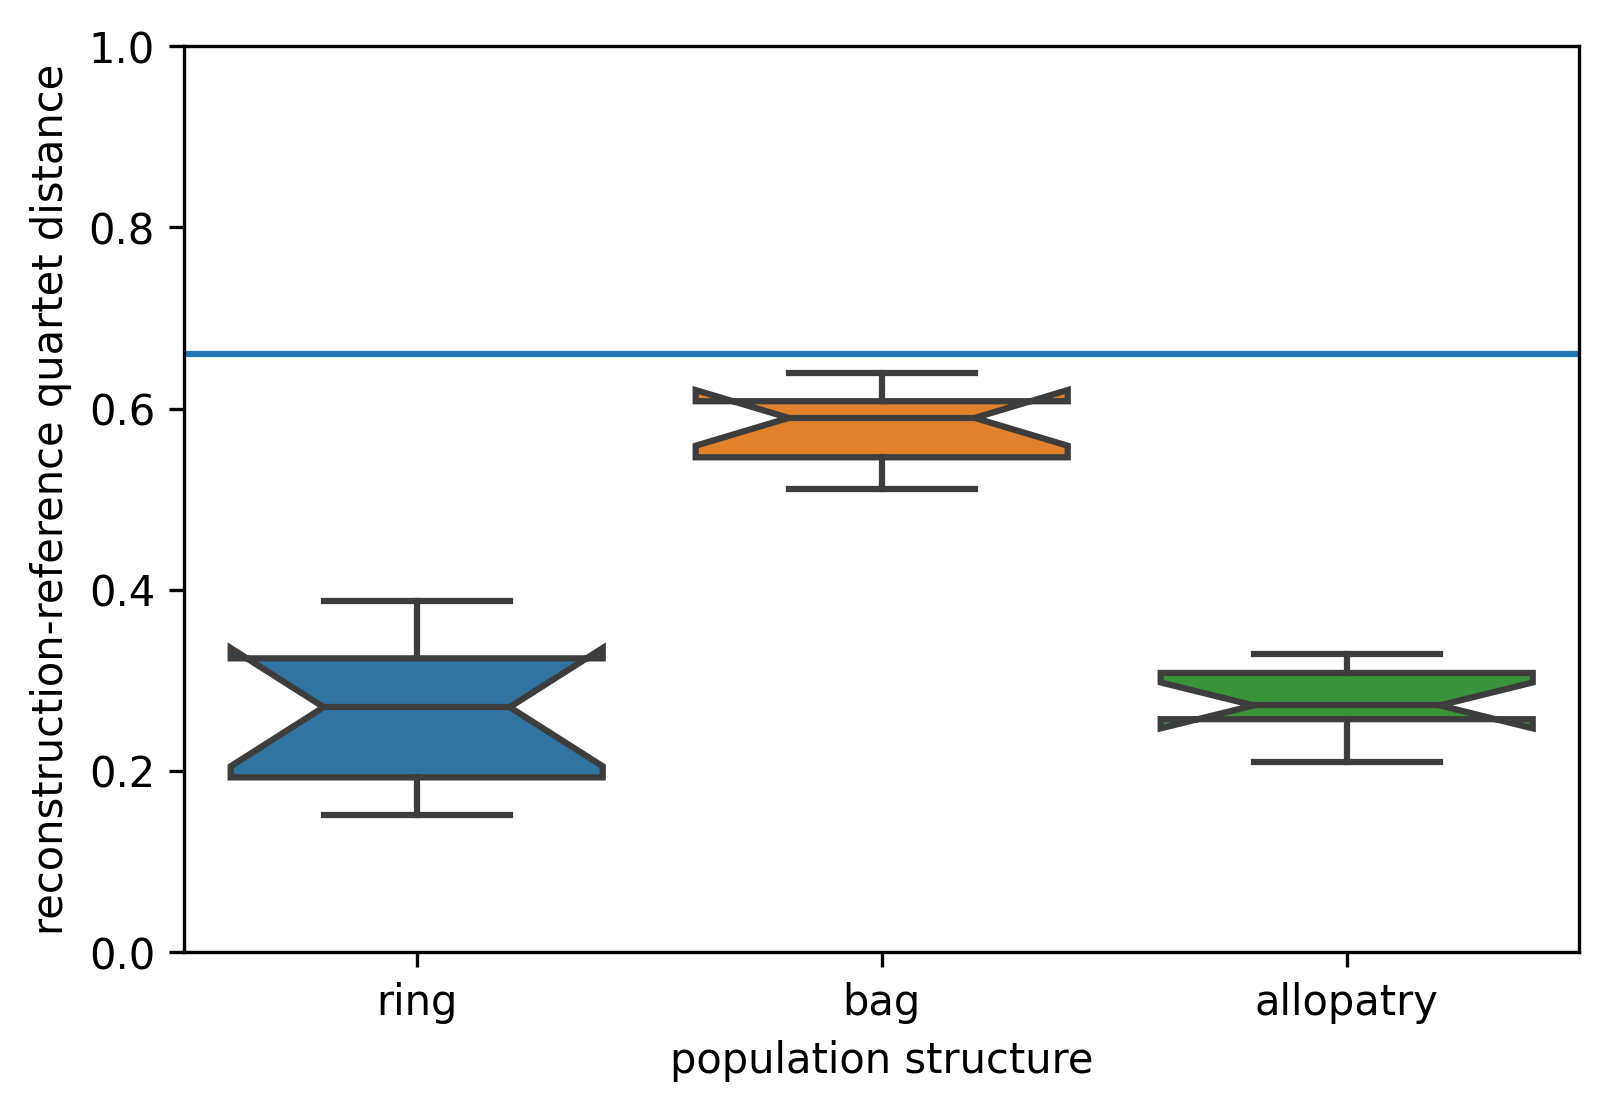
\includegraphics[width=0.8\textwidth]{notebooks/notebooks/teeplots/viz=boxplot-quartet+x=treatment+y=quartet-distance+ext=}
  \caption{
    Normalized quartet distances between reconstructed phylogenies and references distilled from tracked pedigree.
    Lower indicates less reconstruction error.
    Notches give bootstrapped 95\% confidence interval.
    Horizontal blue line indicates expected quartet distance between random trees.
    Some reconstruction error is expected, especially in control treatment, due to resolution of effectively arbitrary phylogenetic structure among well-mixed population components (Section \ref{sec:phylogeny-extraction}).
  }
  \label{fig:species-reconstruction-error}
\end{figure}
